\label{XPS_theory}
\section{X-ray photoelectron spectroscopic analysis}
\subsection{Principle of measurement}
Photoelectron spectroscopy (PES) hinges on the fundamental principle of the photoelectric effect  as elucidated through the photon theory by Einstein and Rutherford \cite{rutherford_xxxvii_1914, einstein_uber_1905}. This concept essentially explains how incident light hitting a material results in the emission of electrons, known as photoelectrons.
In X-ray photoelectron spectroscopy, soft x-rays are commonly generated by exciting Aluminum or Manganese to radiate K \(\alpha\) x-rays with 1486.6 eV and 1253.6 eV respectively. These x-ray sources have a small natural linewidth and thus can provide high resolution. The produced photons then interact with the sample which in turn emit electrons, making use of the photoelectric effect previously described. Those electrons are then transported to a multichannel detector which counts the electrons. To improve, detector efficiency and electron collection, and thus the resolution, a monochromator is usually used.\cite{stevie_introduction_2020} The concept of the measurement can be expressed as shown in eq. 1:
\begin{equation}
    hv = BE + KE + \psi spec
\end{equation}
which can be re-arranged to express the binding energy as a function of known variables \cite{stevie_introduction_2020} as shown in eq. 2
\begin{equation}
    BE = hv- KE - \psi spec
\end{equation}

\begin{figure}
    \centering
    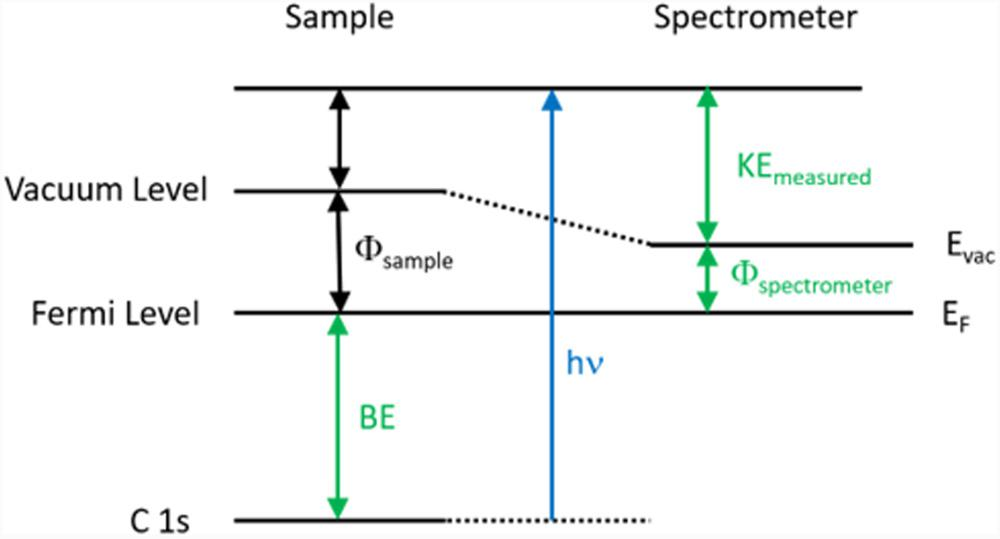
\includegraphics[width=0.7\textwidth]{Figures/image4_3.jpeg}
    \caption{}
    \label{fig:enter-label}
\end{figure}


The sample work function is a specific change in energy levels dependent on the chemical environment (coordination, charge etc.) of the atom of interest. It describes the work an electron must overcome to escape the local environment up to the vacuum level. 



The intensity of the peaks is indicated as counts and corresponds to the number of electrons that reach the detector during the acquisition time. Thus, the intensity of the signal depends on the acquisition time and should be normalized before comparing with spectra collected with unknown method and instrument parameters.
The complex and sample-specific interactions of the produced electrons with the sample are discussed in the next subchapter.

\subsection{Surface sensitivity}

The study of surface sensitivity in XPS has been thoroughly studied and summarized in multiple publications \cite{powell_surface_2009, }. Electrons emitted from the samples atoms can take different ways until they eventually reach the detector. They either take a direct path (A), are elastically scattered and return to the detector (B) or are inelastically scattered and do not return to the detector (C) as shown in \nameref{fig:scattering}.

To this point, there are three terms to describe surface sensitivity in XPS:
\begin{itemize}
\item The initial energy which is needed to overcome dielectric effects such that an electron can be lost from a material is described by the electron loss function (ELF)
\item Inelastic mean free path (IMFP), often denoted as $\lambda$, describes the distance an electron travels in a given material before inelastically scattering.
\item Effective attenuation length (EAL) is the length the electron travels into the sample while also considering elastic scattering effects.

\end{itemize}

\begin{figure}
    \centering
    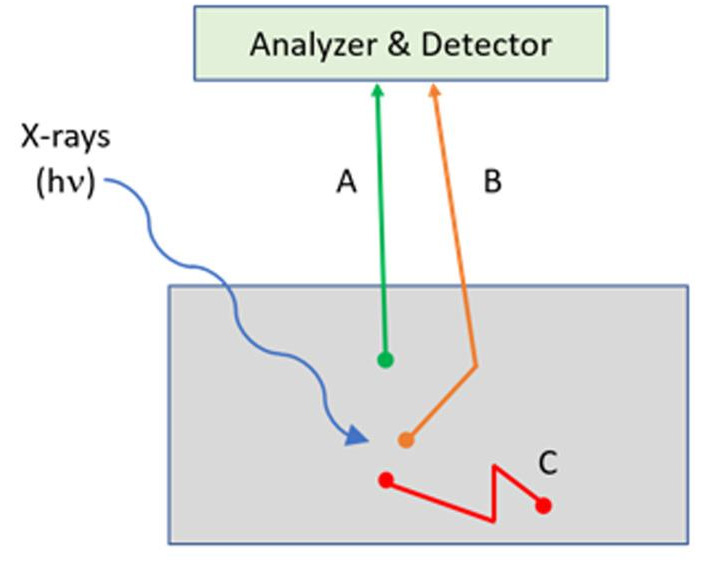
\includegraphics[width=0.3\textwidth]{Figures/image6_1.jpg}
    \caption{Scattering effects in XPS \cite{stevie_introduction_2020}}
    \label{fig:scattering}
\end{figure}

The intensity of electrons emmited from a sample deeper than $d$ can be described using Beer's law as shown in \nameref{beerslaw}.

\begin{equation}
\label{beerslaw}
    I = I_{0} * exp(-d/\lambda)
\end{equation}

Elastic electron scattering (see \nameref{fig:scattering} B), however, has often caused uncertainties in measurements of EAL and IMFP. The IMFP and the EAL are element specific and also depend on the kinetic energy. 
%As the IMFP does not consider elastic scattering, there is a universal curve describing overall tendencies. 
The information depth (ID) is often denoted as 3 $\lambda$, where statistically, 95\% of the information originates. From \nameref{beerslaw}, it is obvious that the information obtained decays non-linearly, 

\subsection{X-ray photoelectron spectra} % identification?
\subsubsection{Direct transitions}
% Photoelectron peaks
As X-ray photoelectron spectroscopy uses x-rays to produce core-level electrons from a sample, the detection of these electrons is the desired origin of a so-called photoelectron peak, which originates in the photoionization effect. The notation for the photoelectron peaks is the element followed by the orbital from which they originate, such as C 1s for the Carbon peak from the 1s orbital \cite{stevie_introduction_2020}. In physical research, cross sections describe the probability of a certain process to take place when a certain material is subject to some radiant excitation. Thus, the photoionization cross section describes the probability of the photoionization process to happen. 

%satellite peaks 
While an electron is travelling towards the detector, it might interact with valence electrons of other atoms and lose some of its energy. This process is an energy-loss process and thus, the peak observed is shifted towards higher binding energy.

%multiplet splitting
A similar effect can be observed for unpaired electrons in the valence bands. The so-called multiplet splitting of photoelectron peaks is shown in \nameref{fig:peaks}.

%Multiplet splitting of core level peaks occurs when there are unpaired electrons in the valence levels and often results in unexpected peak splitting.


\subsubsection{Indirect transitions}
% Auger electron peaks, 
When a core electron is lost due to the X-ray excitation, a deficiency of electrons results. This ionized state is then relaxed with an electron from the outer-most so-called valence orbital \cite{stevie_introduction_2020}. This process induces the release of energy which can then be detected with XPS. It is crucial to note that this process is independent of the source energy and thus, the Auger peak binding energy changes when another source of X-rays is used. This is especially important to resolve issues when Auger peaks overlap with photoelectron peaks.


\begin{figure}[H]
    \centering
    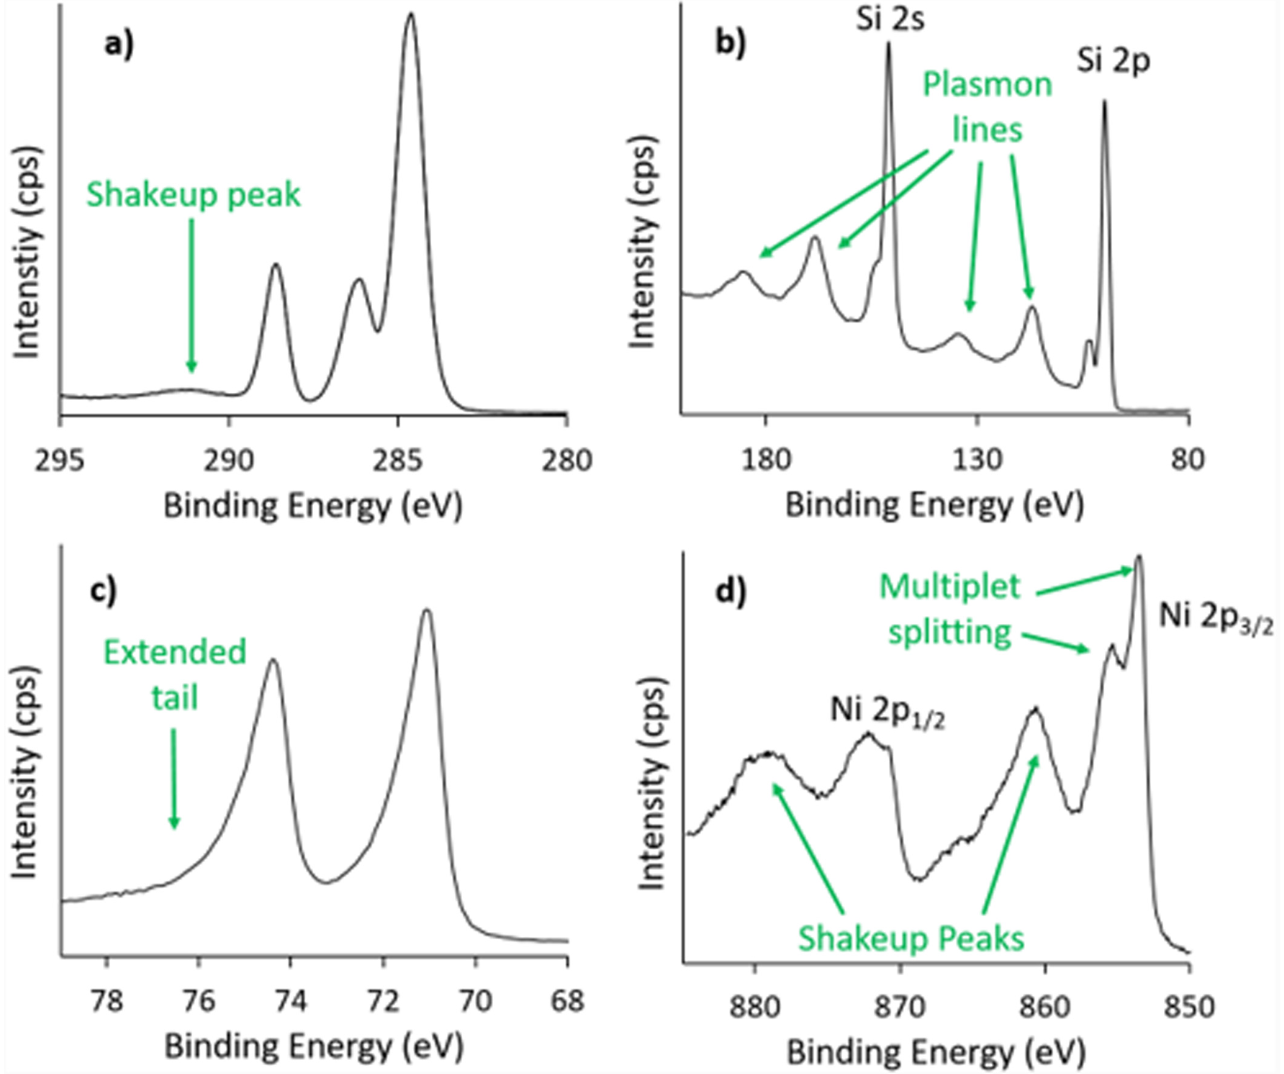
\includegraphics[width=0.75\textwidth]{Figures/peaks.png}
    \caption{Examples of peaks origin (a) C 1s spectrum of PET and its shakeup peak due to the shared $\pi$ electron system, (b) shakeup peaks due to the excitation of Silicon plasmon lines, (c) tailing on a metallic peak due to shakeup excitations (d) Ni 2p from \ch{NiO} - multiplet splitting and shakeup peaks \cite{stevie_introduction_2020}}
    \label{fig:peaks}
\end{figure}


% Plasmon peaks
Plasmon peaks are a special kind of shakeup peaks and arise from the excitation of plasmons. These so-called surface plasmons are formed when electrons from the substrate oscillate due to energy absorption and if the electrons produced by the X-ray source interact with the plasmon, losing kinetic energy. Mostly, this will occur in metals from the first and second group in the periodic table of elements due to the free electrons present that can form plasmons \cite{moulder_handbook_1992}.



\subsection{Adventitious Carbon}
    
When analyzing with XPS, we often find peaks which do not originate from the sample but from the atmosphere. As the atmosphere consists of organic compounds, they include O 1s and C 1s peaks. Often, the C 1s peak is used as a internal standard reference peak to shift the measured spectra to the correct position. This is done because peak shifts occur frequently owing to charging effects which arise from sample properties. Due to varying atmospheric composition, however, this peaks' position is uncertain and is itself  not clearly defined. \cite{biesinger_accessing_2022} As the peak reference to adventitious carbon is most frequently used, it should be considered when comparing, evaluating and analysing experimental data.
In addition, the contamination can be mostly removed when an ion-etching procedure is performed prior to the measurement. Although sometimes referred to as a \emph{contamination layer}, it does not behave similar to a layer, as it is not densely populated on the surface.

\subsection{Quantitative XPS Analysis}
As the quantity of a certain element increases, its corresponding peak should increase as well, given its generated electrons can still escape the sample without being scattered. However, simultaneously, other peaks decrease proportionally in intensity. For example, the peak area of \ch{Al2O3} should sum up to 2:3 for Al:O.
The common procedure for quantitative analysis is to substract the background according to a modelled assumption and subsequently elaborate a relative sensitivity factor (RSF) to measure the area under the peaks and set them into relation.

\subsection{Depth profiling}
In many areas of research, the investigation of surfaces, buried interfaces and quantification in relation to the sample depth is of interest. Experimentally, there exist four methods for investigating depth-information of a component in a sample. These are:
\begin{enumerate}
    \item Presence or absence of energy loss peaks which occur when electrons from deeper regions of the material need to travel to the surface and lose energy (associated to the elastic scattering effect)
    \item The intensity ratio of peaks across the kinetic energy (high vs low) – only suitable for a selection of elements (semi-qualitative).
    \item Controlled erosion and subsequent measurement of the surface (destructive and strong material dependency)
    \item Measurement at different sample-mounting angles (ARXPS). \cite{moulder_handbook_1992} 
    \end{enumerate}
and more recently have been extended by two additional methods:
\begin{enumerate}[resume]
    \item Combination with hard x-ray photoelectron spectroscopy (HAXPES) has become more accessible which in combination with XPS can give depth information of a sample \cite{zborowski_improved_2022}.
    \item Modelling of X-ray photoelectron spectra is another recent technique for the determination of depth distribution and has been investigated previously using manual approaches \cite{zborowski_comparison_2022}.

\end{enumerate}


Methods 1-3 have the drawback of being potentially destructive on the sample surface. Further, they are giving only very vague information about the samples’ depth profile; the accuracy is often denoted to be $\pm$10\%.
The non-destructive methods 4-6 (ARXPS / Modelling / XPS-HAXPES) are further explained, as they are comparable to the data-driven approach used in this work.

\subsubsection{Angle resolved XPS (ARXPS)}
\begin{figure}
    \centering
    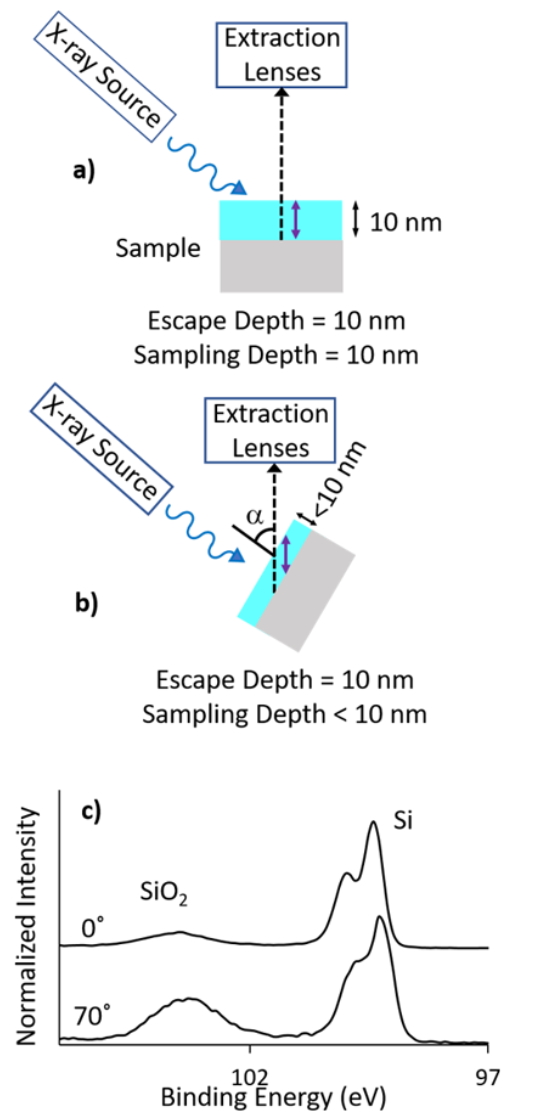
\includegraphics[width=0.4\textwidth]{Figures/ARXPS.png}
    \caption{Angle resolved XPS \cite{stevie_introduction_2020}}
    \label{fig:arxps}
\end{figure}
A variation on the XPS-technique involves measurements at different mounting-angles of the sample.
This changes the path the X-rays take into and out from the sample, as shown in \nameref{fig:arxps} which compares a standard 90\textdegree  take-off angle (a) with a smaller angle $\alpha$ (b). As the angle $\alpha$ decreases, the X-rays travel through a proportional higher amount of surface which in turn increases the sensitivity towards the surface. From the obtained spectra (c), we can deduct the thickness of the layers. This deduction is often done by Software which uses the Maximum entropy method first described by Smith et al. \cite{smith_maximum_1992} in 1992.
The intensity of the peaks in respect to the angle $\alpha$ is shown in \nameref{intensity_angle}, where $G(\alpha)$ is a term representing geometric and instrumental factors and will cancel out as intensity ratios are considered. 
The thickness is denoted as $t$,
$\sigma$ is the photoelectron cross section,
F is the analyzer transmission function,
c is the atomic concentration,
z is the depth and $\lambda$ the IMFP or the EAL
\cite{paynter_arxps_2009}.

\begin{equation}
\label{intensity_angle}
    I_{t} = G(\alpha)\sigma F c \int_{0}^{t} e^{-z/ \lambda cos \alpha} dz
\end{equation}

A newer method collects spectra in parallel, thus is called pARXPS, which reduces acquisition time and constant transmission \cite{bure_assessing_2023}.

\subsubsection{XPS-HAXPES}

Hard X-ray photoelectoron spectroscopy is a technique similar to XPS, but uses Gallium or Chromium to produce hard x-rays to achieve much higher energy levels. As these X-rays are in the range of multiple keVs, the IMFP increases drastically and we are able to probe much deeper into the surface compared to XPS. Combining the two analyses can provide researchers with valuable information of the surface and the deeper regions of samples. This approach has been demonstrated to provide valuable information in multiple publications \cite{bure_assessing_2023, siol_concepts_2020} 

\subsection{Simulation with Sessa}
As XPS spectra are not available from databases in sufficient number for the use as training data in deep learning, we used the NIST Standard Reference Database 100 Software, also called Sessa \cite{noauthor_nist_2010, smekal_simulation_2005}. The development aimed to provide a solution to two main applications - quantitative XPS and simulation of layered samples. The proposed approach for layered systems and thickness analysis is to adjust the model "to find maximum consistency between simulated and measured spectra" \cite{smekal_simulation_2005}.
In Sessa, spectra are simulated using a Monte-Carlo method using the data provided from multiple databases for the following data:

\begin{itemize}
    \item elemental data
    \item differential inverse inelastic mean free path
    \item IMFP values
    \item differential elastic-scattering cross section
    \item total elastic-scattering cross section
    \item transport scattering cross section
    \item photoionization cross section
    \item photoionization asymmetry parameter
    \item electron inner-shell ionization cross section
    \item photoelectron lineshape
    \item binding energies of the elements.
\end{itemize}

Although the exact computational models used in Sessa are not public, Smekal et al. have shown that the linear approximation approach for the angle dependent cross sections, and the depth distribution function (which models surface sensitivity) are in good agreement with experimental data. However, they raise awareness to the need for empirical data in order to realistically model the shape of Auger peaks.